\documentclass[tikz,border=5pt]{standalone}
\usepackage{amsmath}
\usepackage[scaled]{helvet}
\renewcommand{\familydefault}{\sfdefault}
\usetikzlibrary{arrows.meta,calc,positioning}
\definecolor{ink}{HTML}{172033}
\definecolor{muted}{HTML}{667085}
\definecolor{blue}{HTML}{2A78D6}
\definecolor{orange}{HTML}{EB6834}
\definecolor{aqua}{HTML}{1BAF7A}
\definecolor{light}{HTML}{F2F4F7}
\newcommand{\bitcell}[4]{%
  \fill[#3,rounded corners=2pt] (#1,#2) rectangle +(0.62,0.62);
  \draw[#4,line width=.65pt,rounded corners=2pt] (#1,#2) rectangle +(0.62,0.62);
}
\begin{document}
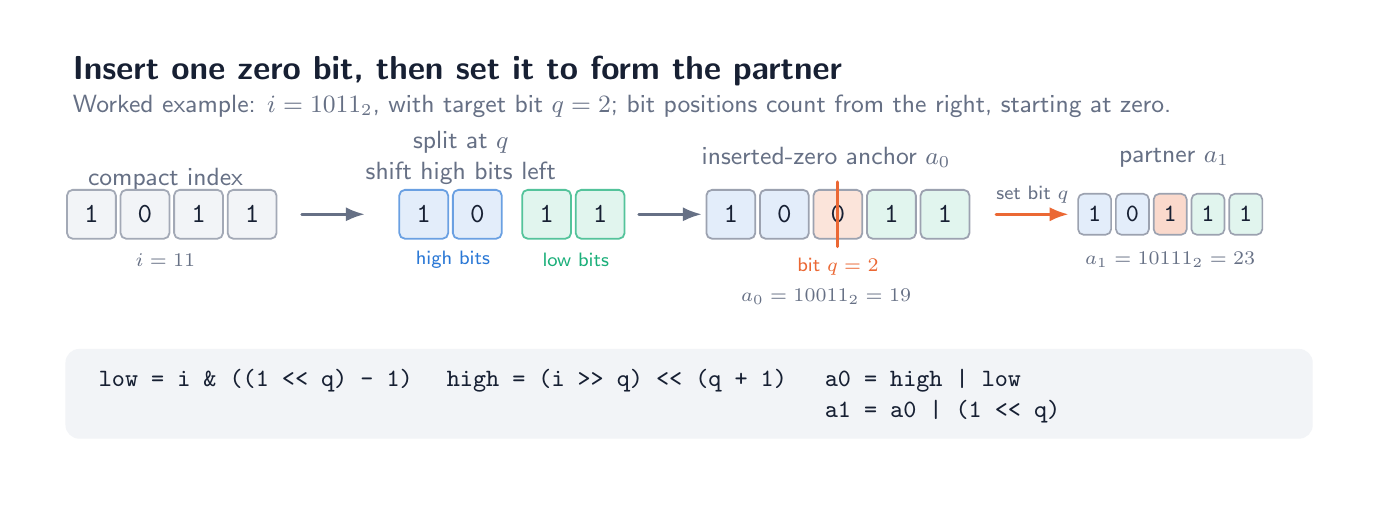
\begin{tikzpicture}[x=1cm,y=1cm,line cap=round,line join=round,font=\sffamily]
  \path[use as bounding box] (0,0) rectangle (16.8,5.7);
  \fill[white] (0,0) rectangle (16.8,5.7);

  \node[anchor=west,text=ink,font=\bfseries\large] at (.45,5.15) {Insert one zero bit, then set it to form the partner};
  \node[anchor=west,text=muted,font=\small] at (.45,4.70) {Worked example: $i=1011_2$, with target bit $q=2$; bit positions count from the right, starting at zero.};

  \node[text=muted,font=\small] at (1.75,3.78) {compact index};
  \foreach \v [count=\k from 0] in {1,0,1,1}{
    \pgfmathsetmacro{\x}{.50+.68*\k}
    \bitcell{\x}{3.02}{light}{muted!60}
    \node[text=ink,font=\ttfamily] at (\x+.31,3.33) {\v};
  }
  \node[text=muted,font=\scriptsize] at (1.75,2.75) {$i=11$};

  \draw[-{Latex[length=2.4mm]},muted,line width=.9pt] (3.48,3.33) -- (4.28,3.33);
  \node[text=muted,font=\small,align=center] at (5.50,4.05) {split at $q$\\shift high bits left};
  \foreach \v [count=\k from 0] in {1,0}{
    \pgfmathsetmacro{\x}{4.72+.68*\k}
    \bitcell{\x}{3.02}{blue!13}{blue!70}
    \node[text=ink,font=\ttfamily] at (\x+.31,3.33) {\v};
  }
  \foreach \v [count=\k from 0] in {1,1}{
    \pgfmathsetmacro{\x}{6.28+.68*\k}
    \bitcell{\x}{3.02}{aqua!13}{aqua!75}
    \node[text=ink,font=\ttfamily] at (\x+.31,3.33) {\v};
  }
  \node[text=blue,font=\scriptsize] at (5.40,2.75) {high bits};
  \node[text=aqua,font=\scriptsize] at (6.96,2.75) {low bits};

  \draw[-{Latex[length=2.4mm]},muted,line width=.9pt] (7.76,3.33) -- (8.56,3.33);
  \node[text=muted,font=\small] at (10.14,4.05) {inserted-zero anchor $a_0$};
  \foreach \v/\c [count=\k from 0] in {1/blue!13,0/blue!13,0/orange!18,1/aqua!13,1/aqua!13}{
    \pgfmathsetmacro{\x}{8.62+.68*\k}
    \bitcell{\x}{3.02}{\c}{muted!65}
    \node[text=ink,font=\ttfamily] at (\x+.31,3.33) {\v};
  }
  \draw[orange,line width=1.1pt] (10.29,2.92) -- (10.29,3.74);
  \node[text=orange,font=\scriptsize] at (10.29,2.66) {bit $q=2$};
  \node[text=muted,font=\scriptsize] at (10.14,2.28) {$a_0=10011_2=19$};

  \draw[-{Latex[length=2.4mm]},orange,line width=1.05pt] (12.30,3.33) -- node[above,text=muted,font=\scriptsize] {set bit $q$} (13.22,3.33);
  \node[text=muted,font=\small] at (14.56,4.05) {partner $a_1$};
  \foreach \v/\c [count=\k from 0] in {1/blue!13,0/blue!13,1/orange!25,1/aqua!13,1/aqua!13}{
    \pgfmathsetmacro{\x}{13.34+.48*\k}
    \fill[\c,rounded corners=2pt] (\x,3.07) rectangle +(0.42,0.52);
    \draw[muted!65,line width=.6pt,rounded corners=2pt] (\x,3.07) rectangle +(0.42,0.52);
    \node[text=ink,font=\ttfamily\small] at (\x+.21,3.33) {\v};
  }
  \node[text=muted,font=\scriptsize] at (14.51,2.75) {$a_1=10111_2=23$};

  \fill[light,rounded corners=5pt] (.48,.48) rectangle (16.32,1.62);
  \node[anchor=west,text=ink,font=\ttfamily\small] at (.78,1.22) {low  = i \& ((1 << q) - 1)};
  \node[anchor=west,text=ink,font=\ttfamily\small] at (5.20,1.22) {high = (i >> q) << (q + 1)};
  \node[anchor=west,text=ink,font=\ttfamily\small] at (10.00,1.22) {a0 = high | low};
  \node[anchor=west,text=ink,font=\ttfamily\small] at (10.00,.82) {a1 = a0 | (1 << q)};
\end{tikzpicture}
\end{document}
